%% A "teaser" image appears between the author and affiliation
%% information and the body of the document, and typically spans the
%% page.
\begin{teaserfigure}
    \subfloat[]{
    \label{fig:teaser:a}
    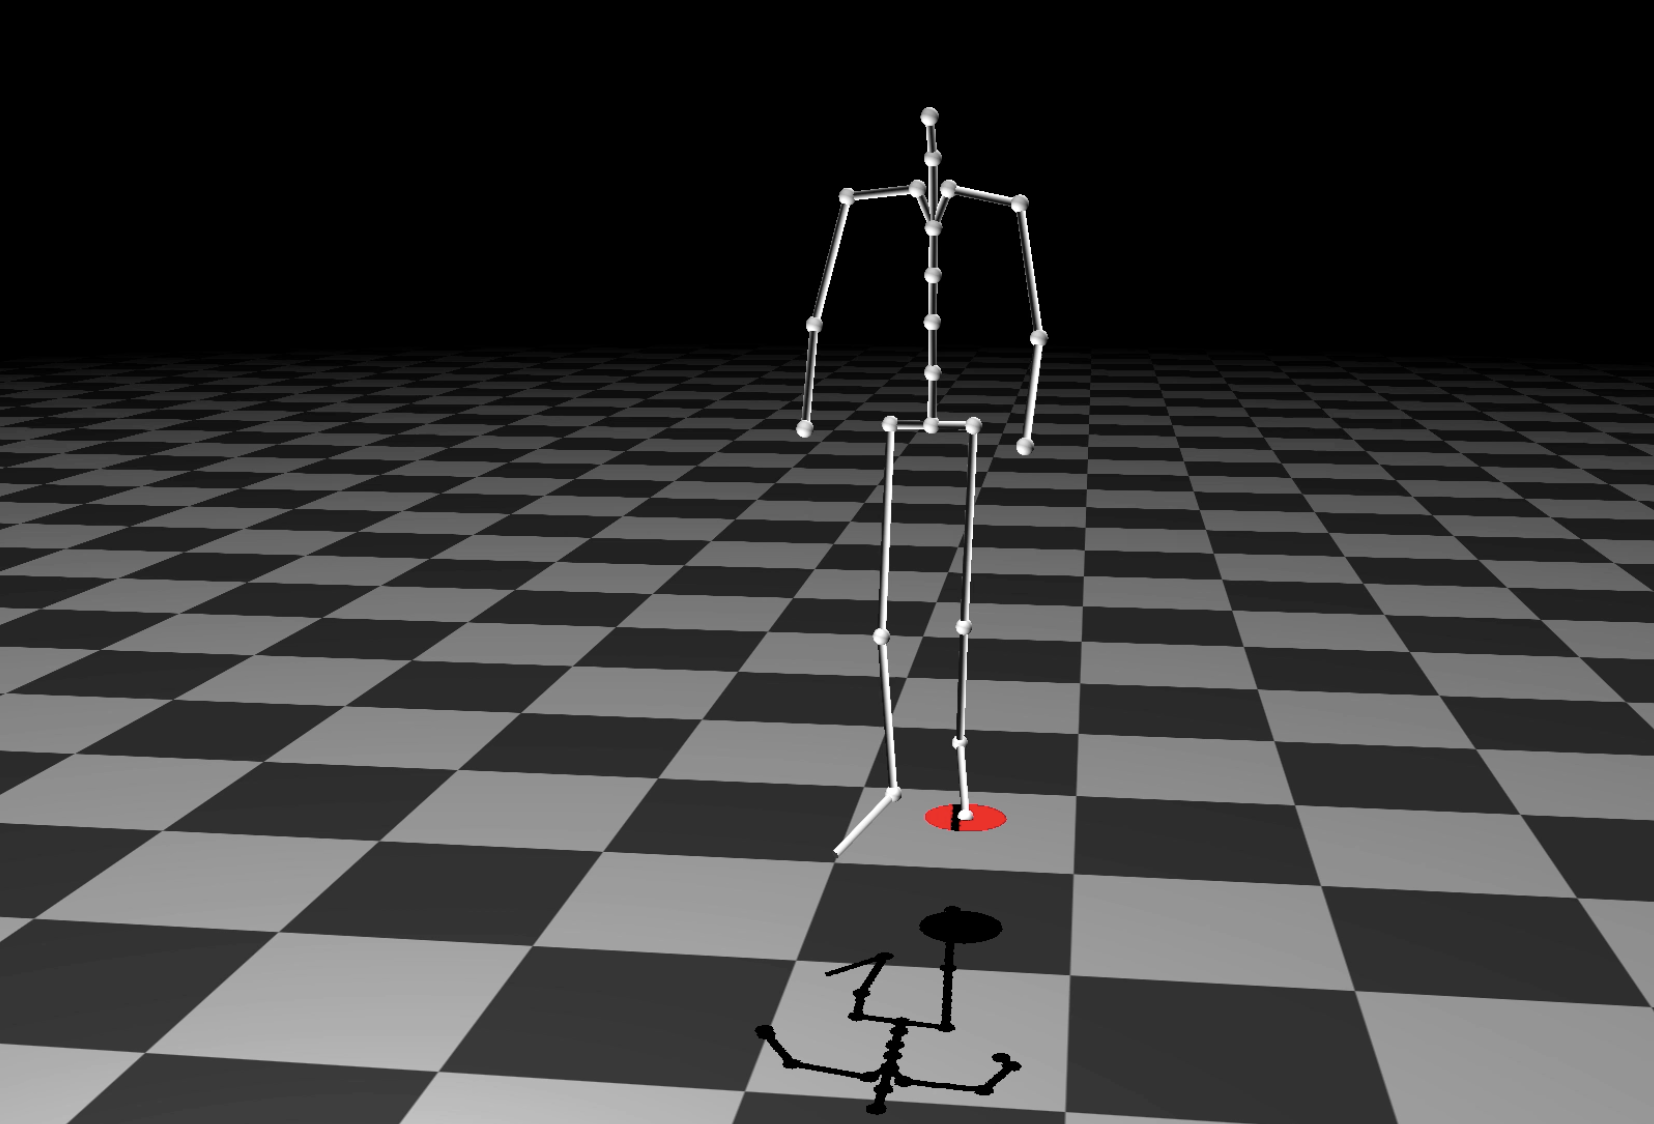
\includegraphics[width=0.25\textwidth]{img/teaser}
    }
    \subfloat[]{
    \label{fig:teaser:b}
        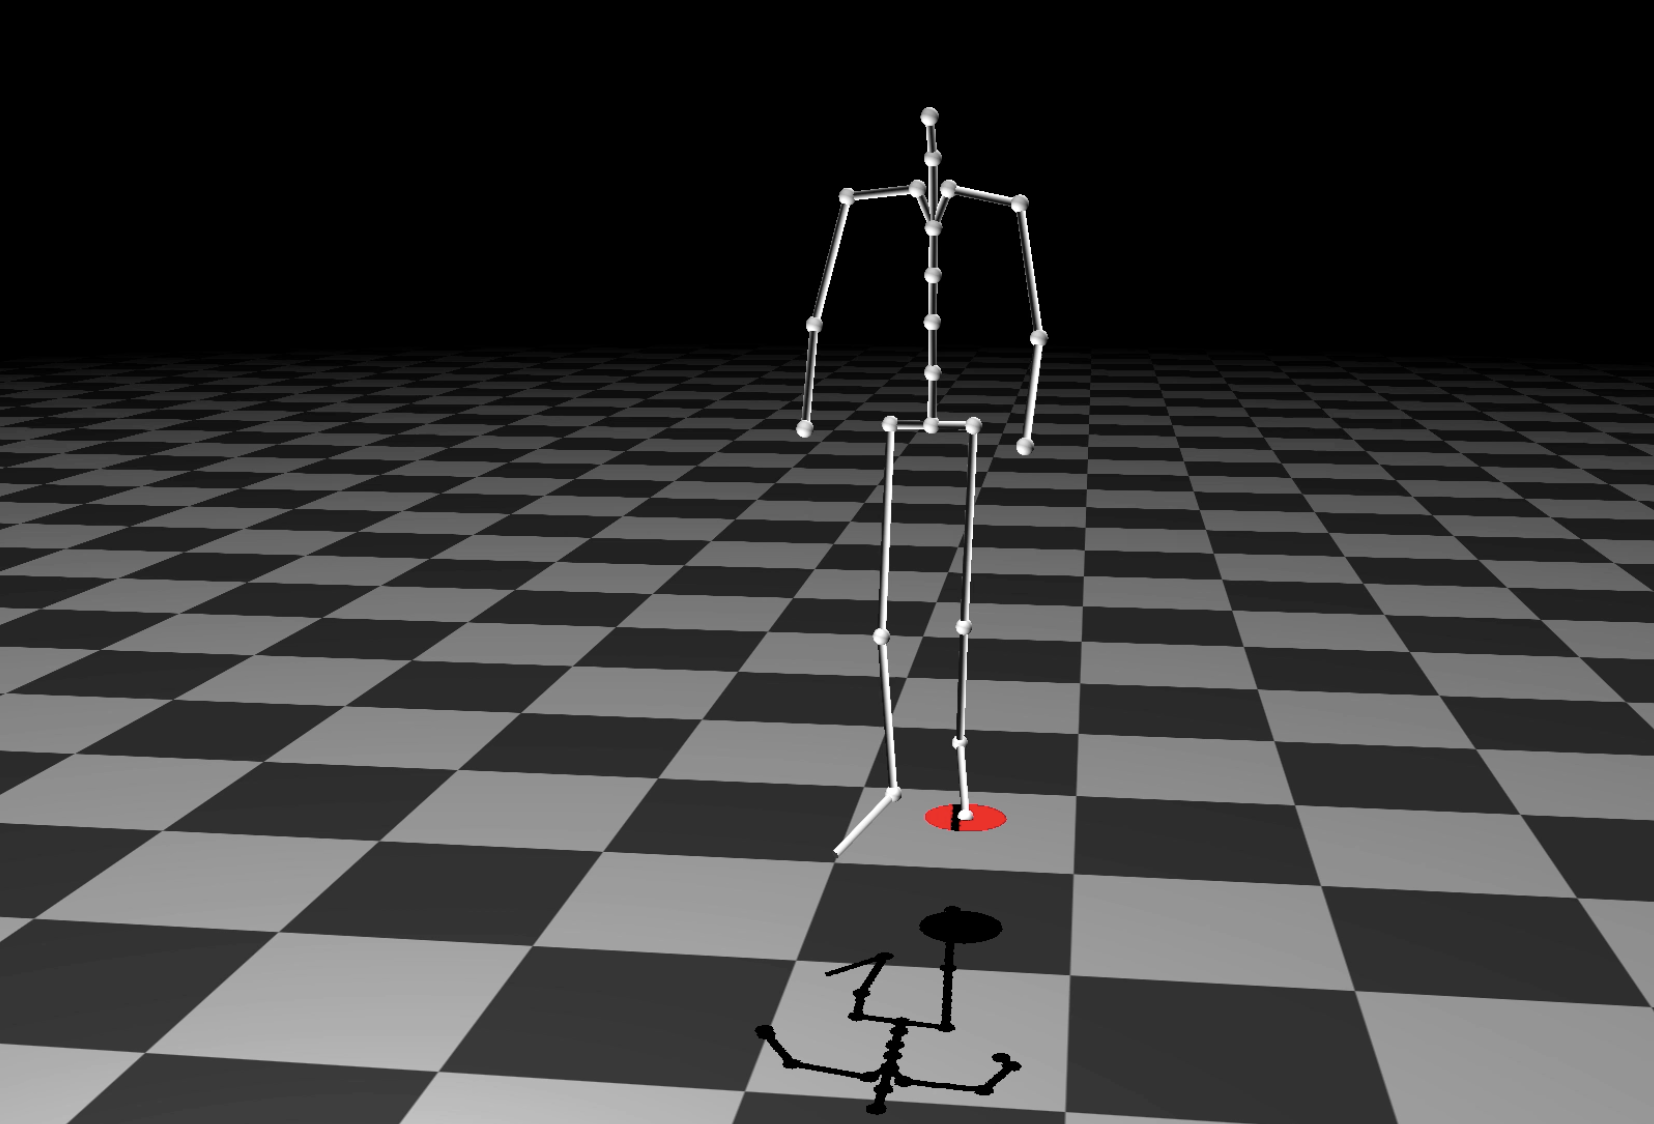
\includegraphics[width=0.25\textwidth]{img/teaser}
    }
    \subfloat[]{
    \label{fig:teaser:c}
    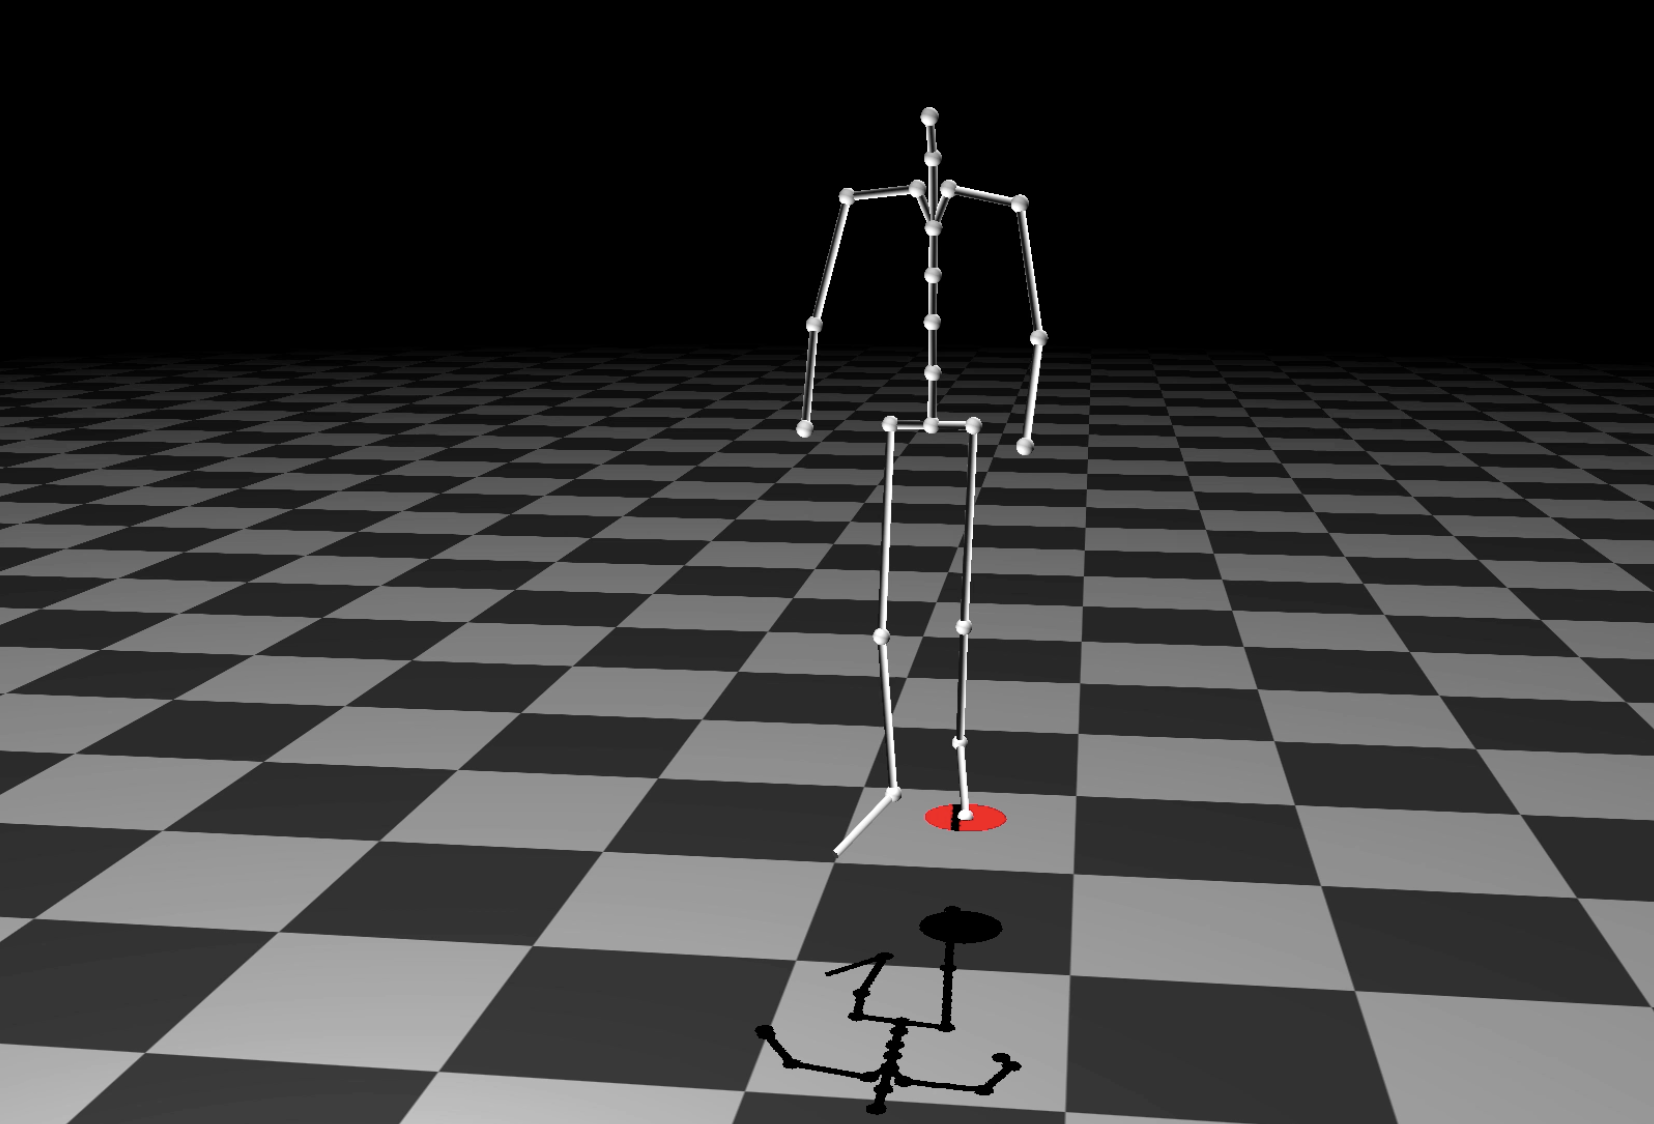
\includegraphics[width=0.25\textwidth]{img/teaser}
    }
    \subfloat[]{
    \label{fig:teaser:d}
    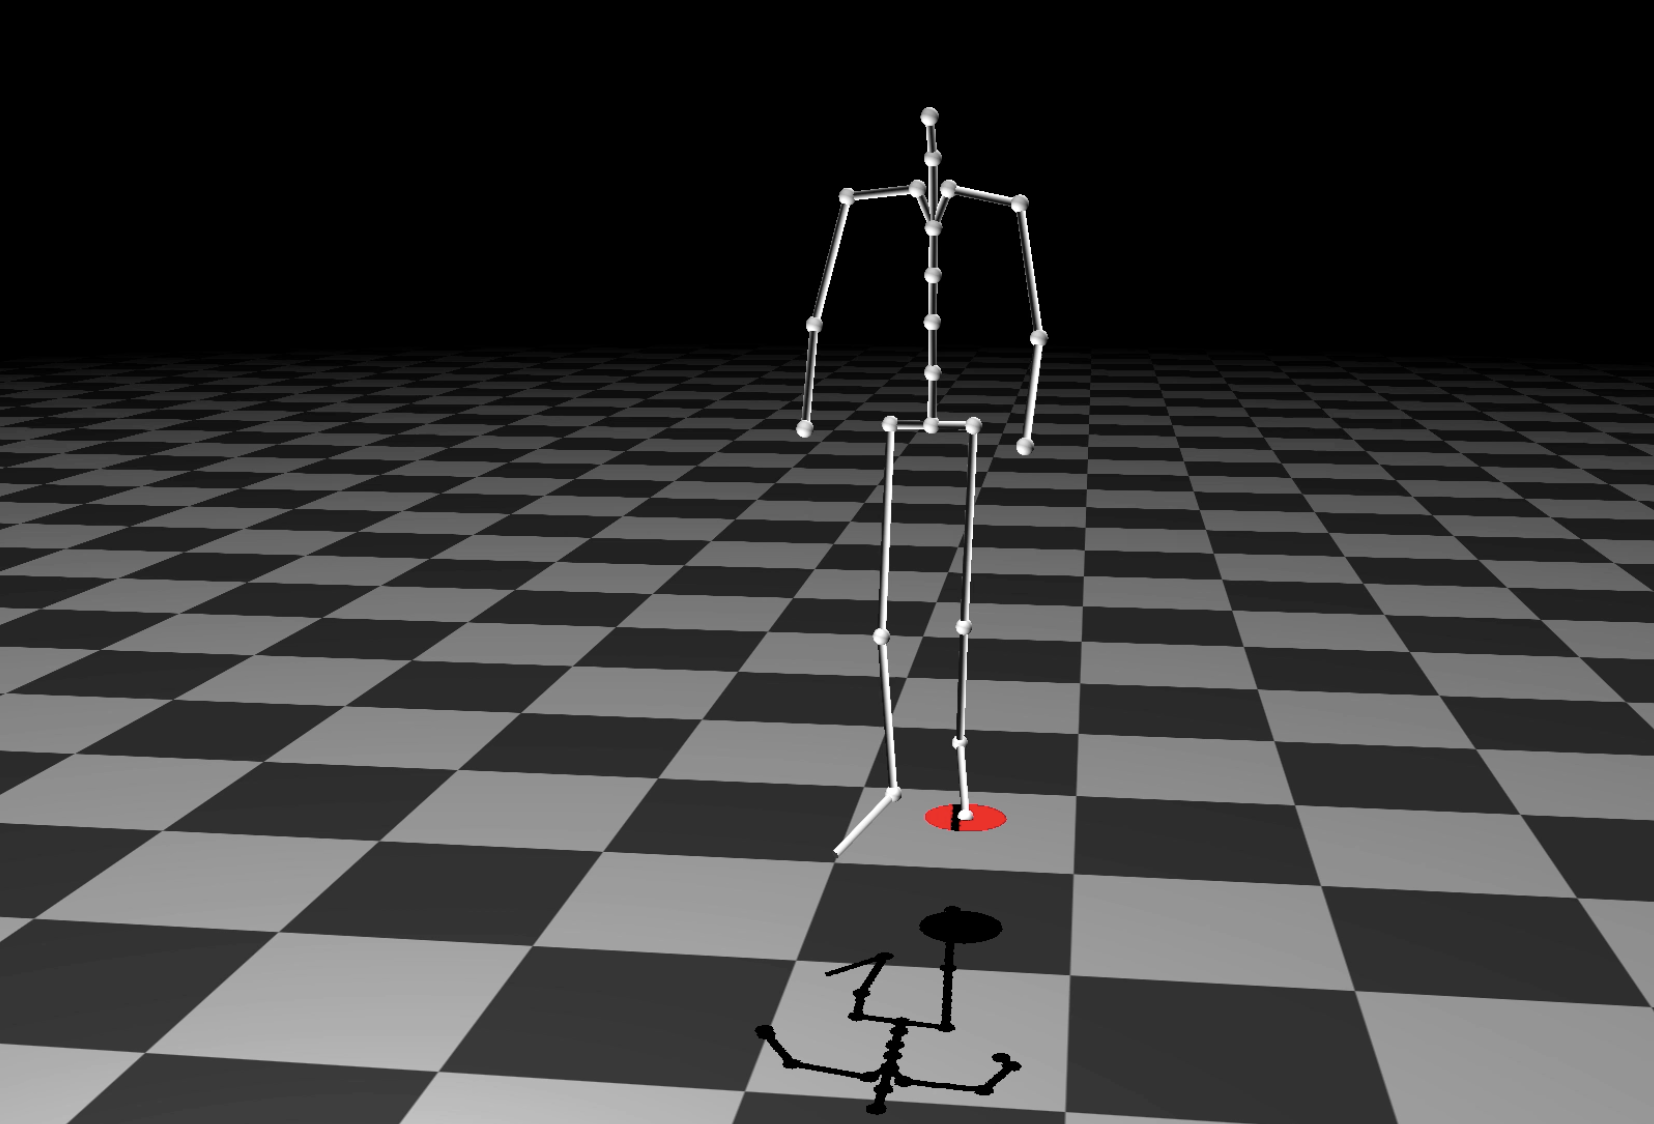
\includegraphics[width=0.25\textwidth]{img/teaser}
    }
    \protect \caption{See my cool graphics illustration of why this is awesome. \protect \subref{fig:teaser:a},\protect \subref{fig:teaser:b},\protect \subref{fig:teaser:c},\protect \subref{fig:teaser:d}.}
  \Description{Awesome.}
  \label{fig:teaser}
\end{teaserfigure}
